\documentclass[conference]{IEEEtran}
\IEEEoverridecommandlockouts
% The preceding line is only needed to identify funding in the first footnote. If that is unneeded, please comment it out.
%Template version as of 6/27/2024

\usepackage{cite}
\usepackage{amsmath,amssymb,amsfonts}
\usepackage{algorithmic}
\usepackage{graphicx}
\usepackage{textcomp}
\usepackage{xcolor}
\usepackage{placeins}

\usepackage{tikz}
\usetikzlibrary{calc, patterns, patterns.meta, shapes.geometric, arrows.meta, positioning, fit}

\usepackage{ifthen}

\usepackage{siunitx} 
\sisetup{locale = US}
\DeclareSIUnit{\Bit}{Bit}

\def\BibTeX{{\rm B\kern-.05em{\sc i\kern-.025em b}\kern-.08em
    T\kern-.1667em\lower.7ex\hbox{E}\kern-.125emX}}

    \begin{document}

\title{Decoding the Amplitude-Modulated Part the DCF77 Longwave Time Signal by using the Goertzel Algorithm}

\author{\IEEEauthorblockN{1\textsuperscript{st} Leander Hackmann}
\IEEEauthorblockA{\textit{Master Embedded Systems Engineering} \\
\textit{FH Dortmund}\\
Dortmund, Germany \\
Mat.-Nr.: 7217912, leander.hackmann001@stud.fh-dortmund.de}
}

\maketitle

\begin{abstract}
    The DCF77, a long wave time signal transmitter that is located near Frankfurt am Main in Germany, is the primary source of time information for
    radio-controlled clocks in Europe. Its signal consists of a phase and an amplitude-modulated part, both containing the time information.
    Devices that use the signal usually consist of an amplitude modulation long wave receiver, often realized by using a dedicated integrated circuit, and an
    application processor. In this paper, an alternative approach for the demodulation of the amplitude-modulated part of the signal, without the need for specialized
    analog cicruitry and only a minimal amount of simple hardware components, is presented.
    This is done by utilizing direct-sampling software-defined radio techniques together with leveraging the efficiency of the Goertzel algorithm.
    As a result, the presented approach removes the need for most of the usually employed analog circuitry, leaving only a front-end amplifier, and therefore
    effectively proposes a new type of design where the receiver is implemented inside the application processor.
    The employed lightweight algorithms keep it realizable on a system with limited resources, which is shown in an example implementation on a Arm Cortex-M3 microcontroller. 
\end{abstract}

\begin{IEEEkeywords}
    DCF77, Goertzel, Digital Signal Processing, Time Signal, Software Defined Radio
\end{IEEEkeywords}

\section{Introduction}
Radio controlled clocks are very popular because they dont require periodical re-adjustment in comparison to common mechanical or quartz-powered clocks.
Instead, the information about the current time is obtained from a RF-signal that is transmitted by an official authority that ensures its availability and
correctness.
The probably most important time signal in Europe is transmitted by the station DCF77 from Mainflingen, a city in Germany that is close to Frankfurt am Main.
The station is operated by a private company that is commissioned by the Physikalisch-Technische Bundesanstalt (PTB) which also supplies the current time information,
generated by two caesium clocks and two caesium fountains. Its operating frequency lies in the long wave area at \SI{77.5}{\kilo\hertz} and the time signal
uses simple modulation techniques (amplitude and phase-modulation) and transmits with \SI{100}{\kilo\watt} Effective Isotropic Radiated Power (EIRP) to enable the reception of the signal in relatively close distances (up to \SI{2000}{\kilo\meter})
with simple technical equipment \cite{b2}.
\begin{figure}[!htbp]
    \centerline{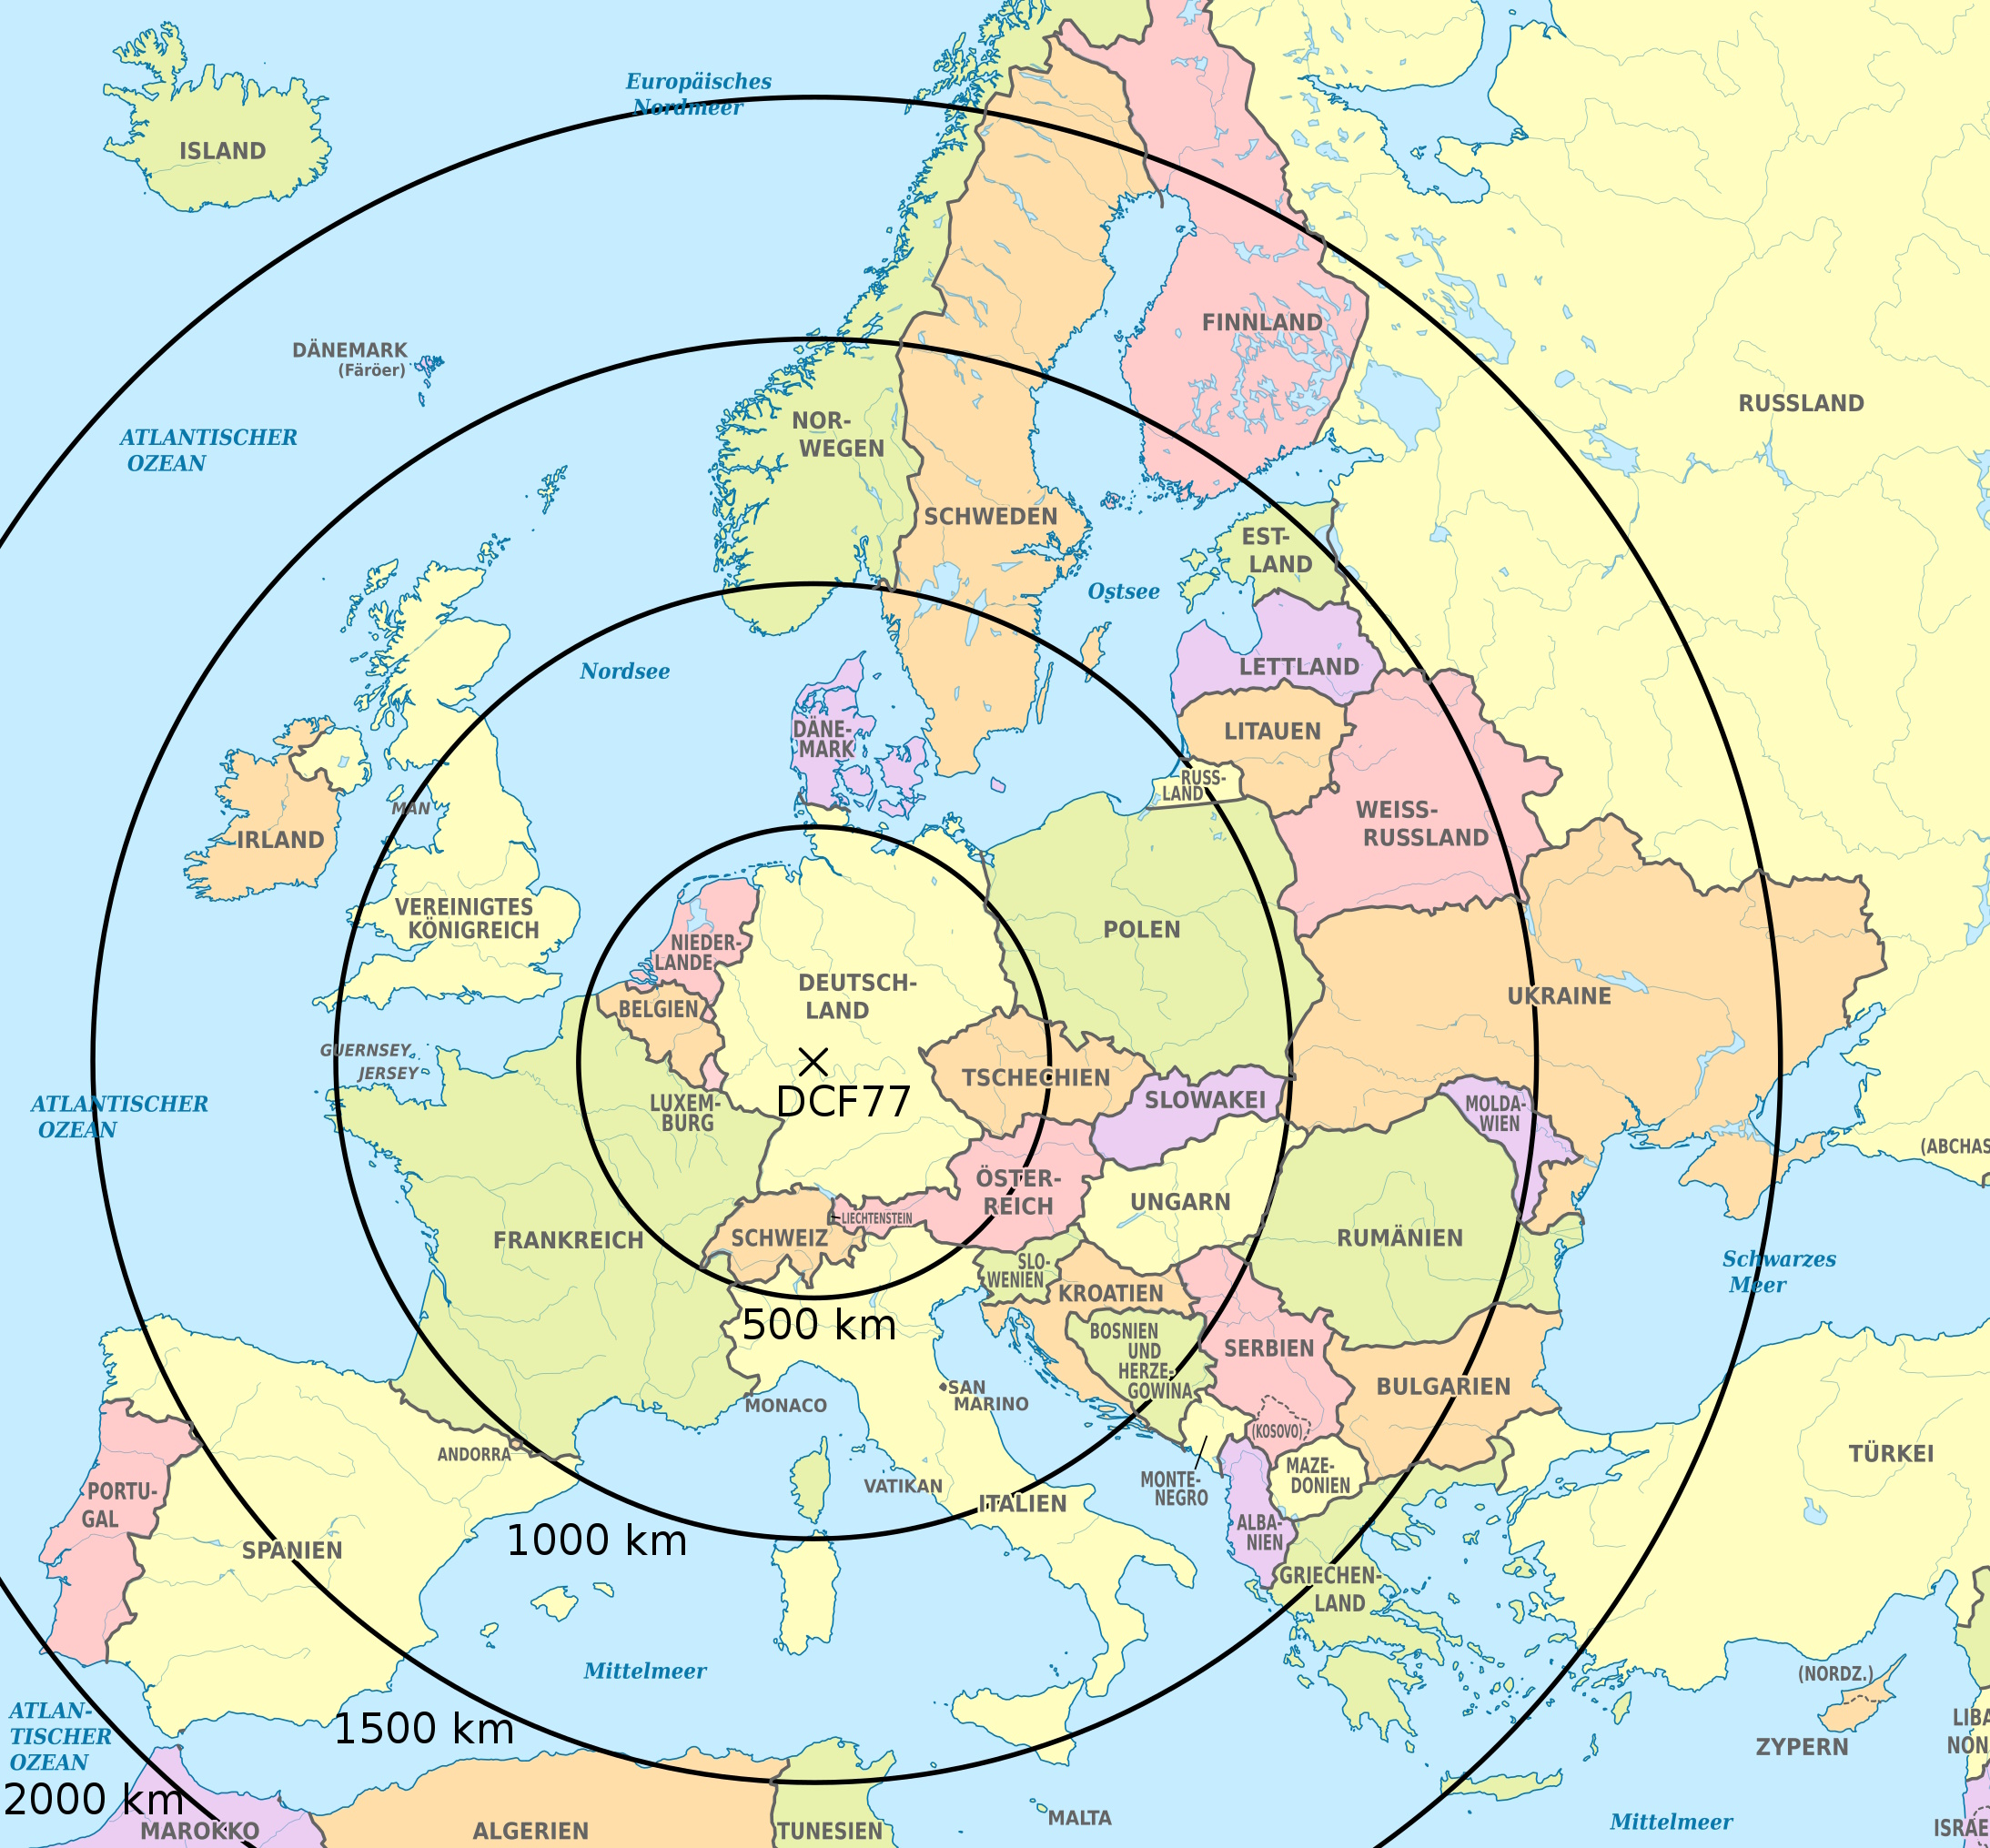
\includegraphics[width=0.3\textwidth]{img/dcf77_range.jpg}}
    \caption{Coverage of the DCF77 signal. Adapted from \cite{b1}}
    \label{fig:dcf77_range}
\end{figure}
\FloatBarrier
End-user devices usually make use of the amplitude-modulated part of the signal by using an amplitude modulation receiver, often a by employing specialized integrated circuit,
together with a rather big ferrite-rod antenna to obtain the time signal.
This time signal then needs further hardware, often in form of a microcontroller used as the applicaton processor, to decode and retrieve the actual time information.
With the increasing availability of computation power and Digital Signal Processing (DSP) capabilities inside cheap mixed-signal microcontrollers, which are already used
to process the time information, the idea to replace to replace the analog receiver portion with a Software Defined Radio (SDR) is more or less obvious.
Moving the receiver into the application processor would allow for a simpler hardware design by shrinking down the complexity and the parts count of the
external analog circuitry. In fact, only a tuned antenna with a basic pre-amplifier is needed.

In this paper, a straightfoward principle for designing a lightweight receiver for the DCF77, based on SDR-techniques, is presented.
After taking a look at the structure of the DCF77 signal, the theoretical operation principle of the receiver is explained and shown in a MATLAB simulation.
To further underline the simplicity and the possibility to implement the principle on a system with limited resources, a demonstration on a Arm Cortex-M3 microcontroller
is shown.

\section{The DCF77 signal}
The DCF77 station operates in the long wave area at a frequency of \SI{77.5}{\kilo\hertz}.
Its operation started with transmitting a frequency standard in 1959.
In 1973, the transmission of the current time information was added to the signal by using amplitude modulation.
To allow a reception under more challenging conditions and with a higher resolution and accuracy, the same time information is also added to the signal since 1983 by using phase-modulation \cite{b3}.
The two different parts of the signal that result out of the parallel amplitude and the phase-modulation can be used for different use-cases that are separated by the
requirements regarding the resolution, accuracy, and the reliability of the obtained time information. 
Whereas the amplitude-modulated part is mainly used for general-purpose time application with low resolution requirements, the phase-modulated part is usually used
for specialized applications that require a higher resolution, accuracy, and reliability.
Although being considered as low in comparison to what is achievable by analyzing the phase-modulated part, the usually observed accuracy uncertainity when using the
amplitude-modulated part it is still well below \SI{1}{\second}, being \SI{100}{\milli\second} \cite{b2}.
When using the phase-modulated part, a standard deviation of \SIrange{\pm 2}{\pm 22}{\micro\second} from the atomic clock to the receving device can be observed \cite{b4}.
\par
As the amplitude-modulated part allows simplistic receiver designs through its straightfoward modulation scheme, it is used in the principle presented in this paper
and therefore a focus is put on explaining this part of the DCF77 signal. The following explainations in this paper therefore refer explicitly to the amplitude-modulated part.
The time information, represented as a series of binary symbols, is modulated onto the carrier with a frequency of \SI{77.5}{\kilo\hertz} by using
Amplitude-Shift Keying (ASK). Every symbol has the duration of exactly \SI{1}{\second}, with a part that is either \SI{100}{\milli\second} or \SI{200}{\milli\second}
long where it has a value to zero.
This the duration of this "gap" is used to encode respectively a 0 or a 1 and effectively switches the strength of the carrier between \SI{15}{\percent} and \SI{100}{\percent} \cite{b5}.
\begin{figure}[htbp]
    \centerline{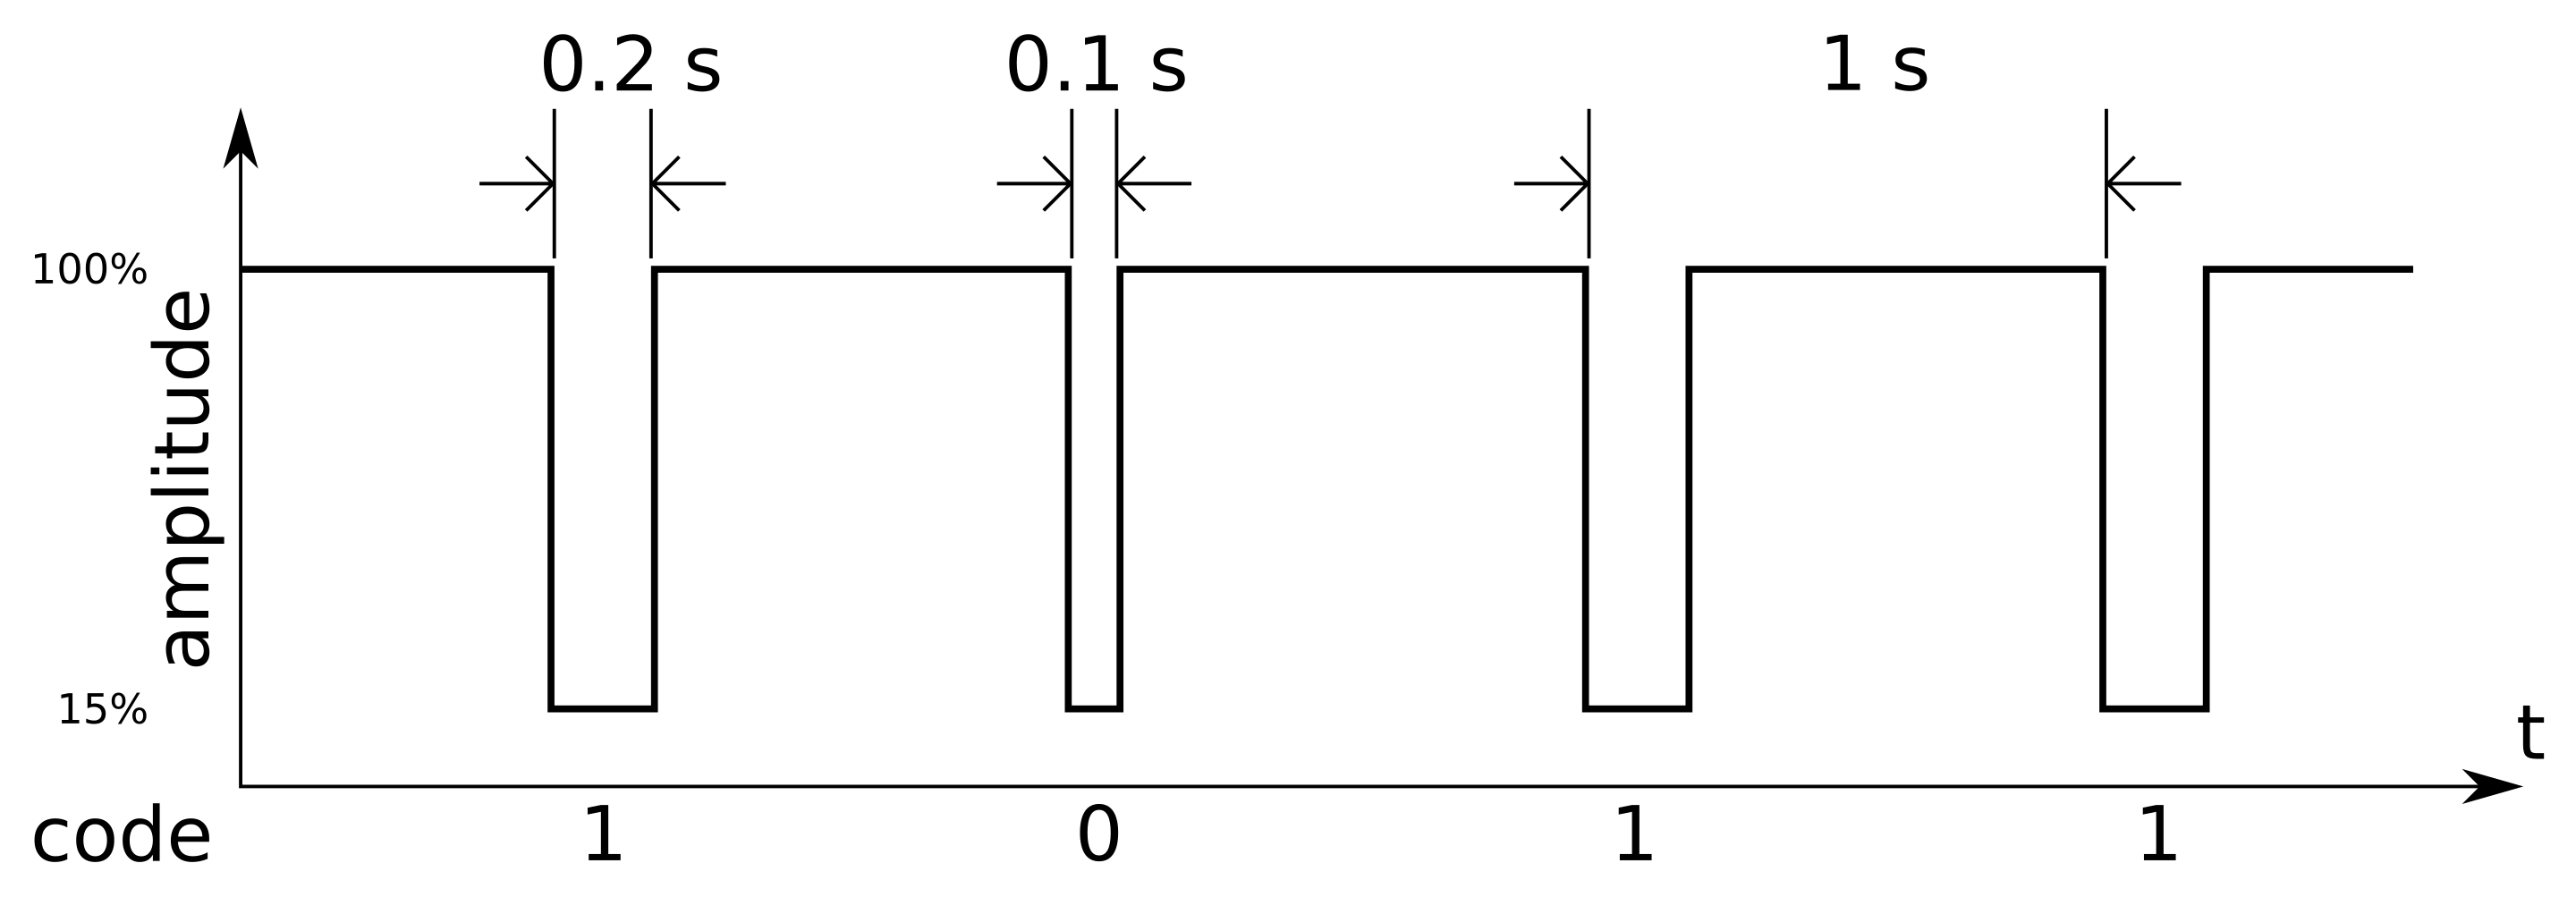
\includegraphics[width=0.45\textwidth]{img/dcf77_symbol_encoding.png}}
    \caption{Symbol encoding of the DCF77 signal. From \cite{b1}}
    \label{fig:dcf77_symbol_encoding}
\end{figure}
\FloatBarrier\noindent
To allow the detection of a new minute, the gap is left out between the last (59) second of the ongoing and the first (0) second of the next minute.
By using this scheme, a dataframe consisting out \SI{59}{\Bit}, starting at second one, can be transmitted every minute.
Bit \SIrange{0}{19}{} are used to send encrypted weather data, to notify the PTB in case of errors in the transmitter, to announce an upcoming
switch to or from Daylight Saving Time (DST), to show if DST is currently enabled or not, and to announce an upcoming leap second \cite{b5}.
As the decryption of the weather date requires a specialized third-party integrated circuit and the notification bit is only important for the PTB, these parts
of the frame are discarded by most applications.
The leftover Bits \SIrange{20}{58}{} are used to represent the current time and date in Binary Coded Decimal (BCD) format, including parity bits for recognizing errors.
\begin{figure}[htbp]
    \centerline{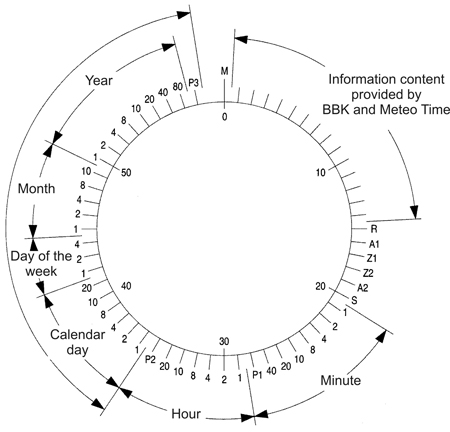
\includegraphics[width=0.35\textwidth]{img/dcf77_frame_encoding.jpg}}
    \caption{Data frame encoding of the DCF77 signal. From \cite{b5}}
    \label{fig:dcf77_data_encoding}
\end{figure}
\FloatBarrier\noindent
This means that a receiver needs to run at least for \SI{39}{\second} after powerup to receive one whole block containing the current time information.
In reality, this period is usually longer because the receiver needs to adapt to the current receiving conditions. 
These conditions underly a lot of influences, including temporary fading, electromagnetic noise from the close environment or varying signal strengths
during different times of the day.

\section{Principle of the receiver}
As the seen in the description of the DCF77 signal, retrieving the the binary time signal from the amplitude-modulated part is more or less trivial.
Conventional applications execute this task by using analog receiving circuits, usually by using a simple amplitude modulation receiver together with a
tuned ferrite-rod antenna, acting as a Bandpass Filter (BPF), to filter out the irrelevant part of the spectrum. 
Moving the receiver into the digital domain allows for more advanced techniques to retrieve this binary time signal, rather than demodulating the signal with a
diode-detector inside the amplitude modulation receiver.
Because the information is contained only in the amplitude of the signal, and therefore inside the signal strength at the receiver, it can also be obtained by doing a
continuous analysis of the spectrum at the carrier's frequency of \SI{77.5}{\kilo\hertz}.
\subsection{The Goertzel Algorithm}
The standard approach to analyze a spectrum in the digital domain after sampling is the well-known Discrete Fourier Transform (DFT), implemented by using
the Fast Fourier Transform (FFT). This yields an analysis of the complete spectrum, producing $\frac{N}{2} + 1$ relevant results for equally distributed frequencies
("frequency bins") within range from \SI{0}{\hertz} to $\frac{f_{s}}{2}$ where $N$ is the number of samples and $f_{s}$ the sampling frequency \cite{b6}.
The signal strength, and therefore the binary time signal of the amplitude-modulated part can then be examined by observing the value of the curresponding frequency bin
over time. Because of only one frequency bin being relevant, it is obvious that a full FFT produces a lot of overhead and redundant calculation operations in this use-case. 
This overhead can be avoided by using the Goertzel algorithm instead of the FFT, which is able to calculate the value of one specific frequency bin with a smaller
amount of needed calculations.
It was invented in 1958 by Gerald Goertzel and since then most commonly used in the detection tones employed in Dual-tone Multi-frequency (DTMF) signaling \cite{b7}.
The working principle of the algorithm can be percieved as a second-order Infinite Impulse Response (IIR) filter where the results $y[n-1]$ and $y[n-2]$ of the output
are stored in states $Q_{1}$ and $Q_{2}$, so they are still available after the execution of the filter.
\begin{equation}
    y[n] = x[n] + 2 \cdot cos(\omega_{g}) \cdot y[n-1] - y[n-2]
\end{equation}
From these equations, the following structure can be derived:
\begin{figure}[htbp]
    \centering
    \resizebox{0.4\textwidth}{!}{
        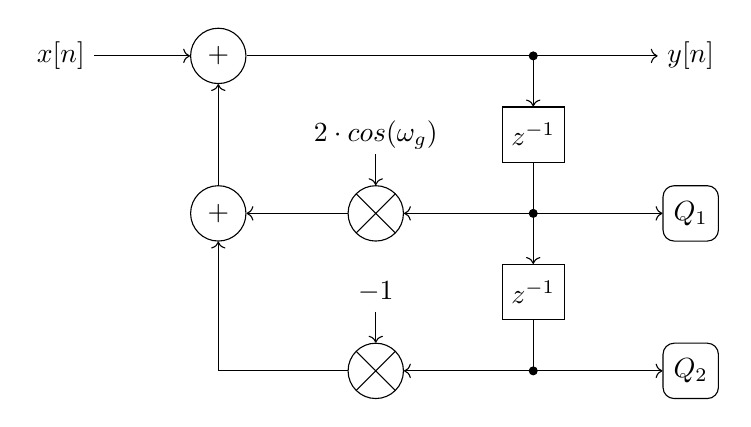
\begin{tikzpicture}[auto, node distance=2cm]
            %Defining a cross set for the multiplication elements
            \tikzset{cross/.style={path picture={ 
            \draw[black]
            (path picture bounding box.south east) -- (path picture bounding box.north west) (path picture bounding box.south west) -- (path picture bounding box.north east);
            }}}
          
          % Define block styles
            \tikzstyle{delay} = [draw, rectangle, minimum height=2em, minimum width=2em]
            \tikzstyle{sum} = [draw, circle, minimum size=2em, node distance=1.5cm]
            \tikzstyle{mult} = [draw, circle, minimum size=2em, node distance=1.5cm, cross]
            \tikzstyle{state} = [draw, rectangle, rounded corners, minimum height=2em, minimum width=2em]
            
            % Nodes
            \node at (-2, 0) (x) {$x[n]$};
            \node[sum] at (0,0) (sum1) {+};
            \node[sum] at (0,-2) (sum2) {+};
            \node[mult] at (2,-2) (mult1) {};
            \node[mult] at (2,-4) (mult2) {};
            \node[delay] at (4,-1) (del1) {$z^{-1}$};
            \node[delay] at (4,-3) (del2) {$z^{-1}$};
            \node[state] at (6,-2) (st1) {$Q_{1}$};
            \node[state] at (6,-4) (st2) {$Q_{2}$};
            \node at (6, 0) (y) {$y[n]$};

            \draw[->] (x.east) -- (sum1.west);
            \draw[->] (sum1.east) -- (y.west);
            \draw[->] (sum2.north) -- (sum1.south);
            \draw[->] (mult1.west) -- (sum2.east);
            \draw[->] (mult2.west) -- (0, -4) -- (sum2.south);
            \draw[->] (4, 0) -- (del1.north);
            \draw[->] (del1.south) -- (del2.north);
            \draw[->] (del2.south) -- (4,-4) -- (mult2.east);
            \draw[->] (4,-2) -- (mult1.east);
            \draw[->] (2, -1.25) -- (mult1.north);
            \draw[->] (2, -3.25) -- (mult2.north);
            \draw[->] (4, -2) -- (st1.west);
            \draw[->] (4, -4) -- (st2.west);
            \node at (2, -1) {$2 \cdot cos(\omega_{g})$};
            \node at (2, -3) {$-1$};
            \node[draw, shape=circle, fill=black, scale=0.3] at (4,0) {};
            \node[draw, shape=circle, fill=black, scale=0.3] at (4,-2) {};
            \node[draw, shape=circle, fill=black, scale=0.3] at (4,-4) {};
        \end{tikzpicture}
    }
\end{figure}
\FloatBarrier\noindent


The constant $2 \cdot cos(\omega_{g})$ is computed before the execution. It is calculated based on $\omega_{g}$ and defines the frequency to be analyzed, dependent on the sampling frequency $f_{s}$, the
frequency to analyze $f_{a}$ and the number of input samples $N$.
\begin{equation}
    k = \left\lfloor \frac{N \cdot f_{a}}{f_{s}} \right\rceil
\end{equation}
\begin{equation}
    w_g = \frac{2\pi \cdot k}{N}
\end{equation}



\begin{figure}[htbp]
    \centering
    \resizebox{0.48\textwidth}{!}{
        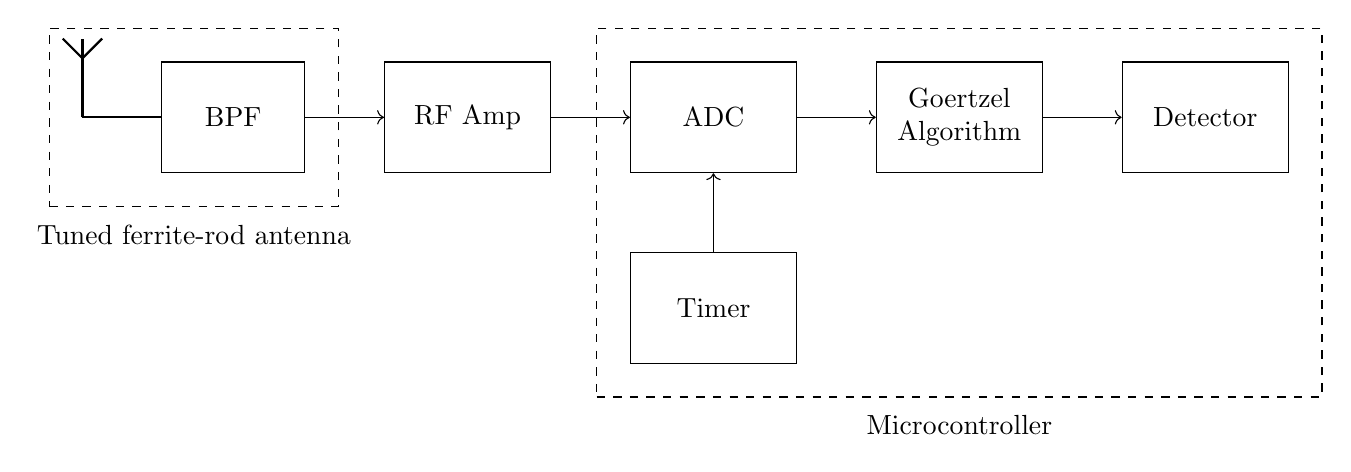
\begin{tikzpicture}
            % Block styles
            \tikzstyle{block} = [rectangle, draw, text width=4.5em, text centered, minimum width=6em, minimum height=4em]
            \tikzstyle{block_dashed} = [rectangle, draw, text width=2em, text centered, minimum width=4em, minimum height=4em, dashed]
            % Input and output
            \begin{scope}[shift={(-3,0)}] % Adjust the position of the antenna
                \coordinate (antenna) at (0,0);
                \draw[thick] (0,0) -- (0,1); % Antenna pole
                \draw[thick] (-0.25,1) -- (0,0.75); % Antenna horizontal line
                \draw[thick] (0.25,1) -- (0,0.75); % Antenna horizontal line
            \end{scope}
            \node[block, right=of antenna, minimum width=4em, minimum height=4em] (bpf) {BPF};
            \node[block, right=of bpf] (rfamp) {RF Amp};
            \node[block, right=of rfamp] (adc) {ADC};
            \node[block, below=of adc] (timer) {Timer};
            \node[block, right=of adc] (goertzel) {Goertzel Algorithm};
            \node[block, right=of goertzel] (det) {Detector};
            % Connections
            \draw[thick] (antenna) -- (bpf);
            \draw[->] (bpf) -- (rfamp); % Connection from antenna to RF amplifier
            \draw[->] (rfamp) -- (adc);
            \draw[->] (timer) -- (adc);
            \draw[->] (adc) -- (goertzel);
            \draw[->] (goertzel) -- (det);

            \node[draw, dashed, fit={(antenna) (bpf)}, inner sep=12pt] (tank_circuit) {};
            \node[below=0.3em of tank_circuit, align=center] {Tuned ferrite-rod antenna};

            \node[draw, dashed, fit={(adc) (timer) (goertzel) (det)}, inner sep=12pt] (microcontroller) {};
            \node[below=0.3em of microcontroller, align=center] {Microcontroller};
        \end{tikzpicture}
    }
\end{figure}
\FloatBarrier\noindent
Test

\begin{figure*}[!htbp]
    \centering
    \resizebox{0.9\textwidth}{!}{
        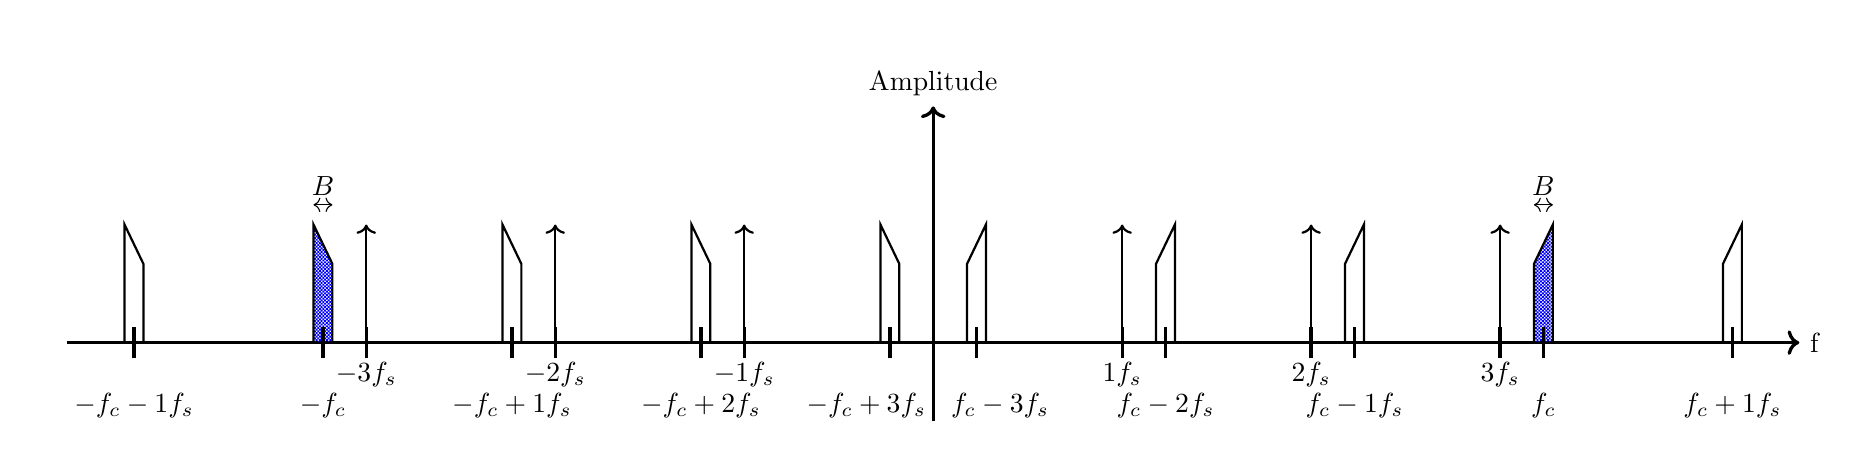
\begin{tikzpicture}
            \clip (-11.5,-1) rectangle + (23,5); %Clipping: where to start, shape and size
            
            \coordinate (fc) at (7.75,0);
            \coordinate (fs) at (2.4,0);
            
            %Axes
            \draw[->, very thick] (-11,0) -- (11,0) node[right] {f};
            \draw[->, very thick] (0,-1) -- (0,3) node[above] {Amplitude};
            
            %DCF77 at f_c
            \draw[thick, pattern={Dots[angle=45,distance={1.25pt/sqrt(2)}]}, pattern color=blue]
            ($(fc) + (-0.12,0)$) -- % Left line start
            ++(0,1) -- %Left line up
            ++(0.24,0.5) -- %Roof
            ++(0,-1.5) -- %Right line down
            cycle; % Close the shape
            \draw[very thick] ($(fc) + (0, -0.2)$) -- ++(0, 0.4); %Line x-axis
            \node at ($(fc) + (0, -0.8)$) {$f_{c}$}; %Index x-axis
            \draw[<->] ($(fc) + (-0.12,1.75)$) -- ++(0.24,0) node[midway, above] {$B$}; %Bandwidth

            %DCF77 at f_c
            \draw[thick, pattern={Dots[angle=45,distance={1.25pt/sqrt(2)}]}, pattern color=blue]
            ($-1*(fc) + (-0.12,0)$) -- % Left line start
            ++(0,1.5) -- %Left line up
            ++(0.24,-0.5) -- %Roof
            ++(0,-1) -- %Right line down
            cycle; % Close the shape
            \draw[very thick] ($-1*(fc) + (0, -0.2)$) -- ++(0, 0.4); %Line x-axis
            \node at ($-1*(fc) + (0, -0.8)$) {$-f_{c}$}; %Index x-axis
            \draw[<->] ($-1*(fc) + (-0.12,1.75)$) -- ++(0.24,0) node[midway, above] {$B$}; %Bandwidth

            %f_s their result of the convulutions
            \foreach \x in {-3,-2,-1,1,2,3}{
                \draw[-> , thick] ($\x*(fs)$) -- ++(0,1.5);
                \draw[very thick] ($\x*(fs) + (0,-0.2)$) -- ++(0,0.4);
                \node at ($\x*(fs) + (0,-0.4)$) {$\x f_{s}$};
                
                
                \draw[thick]
                ($(fc) + (-0.12,0) + \x*(fs)$) -- % Left line start
                ++(0,1) -- %Left line up
                ++(0.24,0.5) -- %Roof
                ++(0,-1.5) -- %Right line down
                cycle; % Close the shape
                \draw[very thick] ($(fc) + (0, -0.2) + \x*(fs)$) -- ++(0, 0.4); %Line x-axis
                \ifthenelse{\x = -3}{
                    \node at ($(fc) + (0.3, -0.8) + \x*(fs)$) {$f_{c} \pgfmathprintnumber[print sign]{\x} f_{s}$}; %Index x-axis
                }{
                    \node at ($(fc) + (0, -0.8) + \x*(fs)$) {$f_{c} \pgfmathprintnumber[print sign]{\x} f_{s}$}; %Index x-axis
                }
        
                %DCF77 at -f_c
                \draw[thick]
                ($-1*(fc) + (-0.12,0) + \x*(fs)$) -- % Left line start
                ++(0,1.5) -- %Left line up
                ++(0.24,-0.5) -- %Roof
                ++(0,-1) -- %Right line down
                cycle; % Close the shape
                \draw[very thick] ($-1*(fc) + (0, -0.2) + \x*(fs)$) -- ++(0, 0.4); %Line x-axis
                \ifthenelse{\x = 3}{
                    \node at ($-1*(fc) + (-0.3, -0.8) + \x*(fs)$) {$-f_{c} \pgfmathprintnumber[print sign]{\x} f_{s}$}; %Index x-axis
                }{
                    \node at ($-1*(fc) + (0, -0.8) + \x*(fs)$) {$-f_{c} \pgfmathprintnumber[print sign]{\x} f_{s}$}; %Index x-axis
                }
            };
        \end{tikzpicture}
    } 
\end{figure*}   


\subsection{Maintaining the Integrity of the Specifications}

The IEEEtran class file is used to format your paper and style the text. All margins, 
column widths, line spaces, and text fonts are prescribed; please do not 
alter them. You may note peculiarities. For example, the head margin
measures proportionately more than is customary. This measurement 
and others are deliberate, using specifications that anticipate your paper 
as one part of the entire proceedings, and not as an independent document. 
Please do not revise any of the current designations.

\section{Prepare Your Paper Before Styling}
Before you begin to format your paper, first write and save the content as a 
separate text file. Complete all content and organizational editing before 
formatting. Please note sections \ref{AA} to \ref{FAT} below for more information on 
proofreading, spelling and grammar.

Keep your text and graphic files separate until after the text has been 
formatted and styled. Do not number text heads---{\LaTeX} will do that 
for you.

\subsection{Abbreviations and Acronyms}\label{AA}
Define abbreviations and acronyms the first time they are used in the text, 
even after they have been defined in the abstract. Abbreviations such as 
IEEE, SI, MKS, CGS, ac, dc, and rms do not have to be defined. Do not use 
abbreviations in the title or heads unless they are unavoidable.

\subsection{Units}
\begin{itemize}
\item Use either SI (MKS) or CGS as primary units. (SI units are encouraged.) English units may be used as secondary units (in parentheses). An exception would be the use of English units as identifiers in trade, such as ``3.5-inch disk drive''.
\item Avoid combining SI and CGS units, such as current in amperes and magnetic field in oersteds. This often leads to confusion because equations do not balance dimensionally. If you must use mixed units, clearly state the units for each quantity that you use in an equation.
\item Do not mix complete spellings and abbreviations of units: ``Wb/m\textsuperscript{2}'' or ``webers per square meter'', not ``webers/m\textsuperscript{2}''. Spell out units when they appear in text: ``. . . a few henries'', not ``. . . a few H''.
\item Use a zero before decimal points: ``0.25'', not ``.25''. Use ``cm\textsuperscript{3}'', not ``cc''.)
\end{itemize}

\subsection{Equations}
Number equations consecutively. To make your 
equations more compact, you may use the solidus (~/~), the exp function, or 
appropriate exponents. Italicize Roman symbols for quantities and variables, 
but not Greek symbols. Use a long dash rather than a hyphen for a minus 
sign. Punctuate equations with commas or periods when they are part of a 
sentence, as in:
\begin{equation}
a+b=\gamma\label{eq}
\end{equation}

Be sure that the 
symbols in your equation have been defined before or immediately following 
the equation. Use ``\eqref{eq}'', not ``Eq.~\eqref{eq}'' or ``equation \eqref{eq}'', except at 
the beginning of a sentence: ``Equation \eqref{eq} is . . .''

\subsection{\LaTeX-Specific Advice}

Please use ``soft'' (e.g., \verb|\eqref{Eq}|) cross references instead
of ``hard'' references (e.g., \verb|(1)|). That will make it possible
to combine sections, add equations, or change the order of figures or
citations without having to go through the file line by line.

Please don't use the \verb|{eqnarray}| equation environment. Use
\verb|{align}| or \verb|{IEEEeqnarray}| instead. The \verb|{eqnarray}|
environment leaves unsightly spaces around relation symbols.

Please note that the \verb|{subequations}| environment in {\LaTeX}
will increment the main equation counter even when there are no
equation numbers displayed. If you forget that, you might write an
article in which the equation numbers skip from (17) to (20), causing
the copy editors to wonder if you've discovered a new method of
counting.

{\BibTeX} does not work by magic. It doesn't get the bibliographic
data from thin air but from .bib files. If you use {\BibTeX} to produce a
bibliography you must send the .bib files. 

{\LaTeX} can't read your mind. If you assign the same label to a
subsubsection and a table, you might find that Table I has been cross
referenced as Table IV-B3. 

{\LaTeX} does not have precognitive abilities. If you put a
\verb|\label| command before the command that updates the counter it's
supposed to be using, the label will pick up the last counter to be
cross referenced instead. In particular, a \verb|\label| command
should not go before the caption of a figure or a table.

Do not use \verb|\nonumber| inside the \verb|{array}| environment. It
will not stop equation numbers inside \verb|{array}| (there won't be
any anyway) and it might stop a wanted equation number in the
surrounding equation.

\subsection{Some Common Mistakes}\label{SCM}
\begin{itemize}
\item The word ``data'' is plural, not singular.
\item The subscript for the permeability of vacuum $\mu_{0}$, and other common scientific constants, is zero with subscript formatting, not a lowercase letter ``o''.
\item In American English, commas, semicolons, periods, question and exclamation marks are located within quotation marks only when a complete thought or name is cited, such as a title or full quotation. When quotation marks are used, instead of a bold or italic typeface, to highlight a word or phrase, punctuation should appear outside of the quotation marks. A parenthetical phrase or statement at the end of a sentence is punctuated outside of the closing parenthesis (like this). (A parenthetical sentence is punctuated within the parentheses.)
\item A graph within a graph is an ``inset'', not an ``insert''. The word alternatively is preferred to the word ``alternately'' (unless you really mean something that alternates).
\item Do not use the word ``essentially'' to mean ``approximately'' or ``effectively''.
\item In your paper title, if the words ``that uses'' can accurately replace the word ``using'', capitalize the ``u''; if not, keep using lower-cased.
\item Be aware of the different meanings of the homophones ``affect'' and ``effect'', ``complement'' and ``compliment'', ``discreet'' and ``discrete'', ``principal'' and ``principle''.
\item Do not confuse ``imply'' and ``infer''.
\item The prefix ``non'' is not a word; it should be joined to the word it modifies, usually without a hyphen.
\item There is no period after the ``et'' in the Latin abbreviation ``et al.''.
\item The abbreviation ``i.e.'' means ``that is'', and the abbreviation ``e.g.'' means ``for example''.
\end{itemize}
An excellent style manual for science writers is \cite{b7}.

\subsection{Authors and Affiliations}\label{AAA}
\textbf{The class file is designed for, but not limited to, six authors.} A 
minimum of one author is required for all conference articles. Author names 
should be listed starting from left to right and then moving down to the 
next line. This is the author sequence that will be used in future citations 
and by indexing services. Names should not be listed in columns nor group by 
affiliation. Please keep your affiliations as succinct as possible (for 
example, do not differentiate among departments of the same organization).

\subsection{Identify the Headings}\label{ITH}
Headings, or heads, are organizational devices that guide the reader through 
your paper. There are two types: component heads and text heads.

Component heads identify the different components of your paper and are not 
topically subordinate to each other. Examples include Acknowledgments and 
References and, for these, the correct style to use is ``Heading 5''. Use 
``figure caption'' for your Figure captions, and ``table head'' for your 
table title. Run-in heads, such as ``Abstract'', will require you to apply a 
style (in this case, italic) in addition to the style provided by the drop 
down menu to differentiate the head from the text.

Text heads organize the topics on a relational, hierarchical basis. For 
example, the paper title is the primary text head because all subsequent 
material relates and elaborates on this one topic. If there are two or more 
sub-topics, the next level head (uppercase Roman numerals) should be used 
and, conversely, if there are not at least two sub-topics, then no subheads 
should be introduced.

\subsection{Figures and Tables}\label{FAT}
\paragraph{Positioning Figures and Tables} Place figures and tables at the top and 
bottom of columns. Avoid placing them in the middle of columns. Large 
figures and tables may span across both columns. Figure captions should be 
below the figures; table heads should appear above the tables. Insert 
figures and tables after they are cited in the text. Use the abbreviation 
``Fig.~\ref{fig}'', even at the beginning of a sentence.

\begin{table}[htbp]
\caption{Table Type Styles}
\begin{center}
\begin{tabular}{|c|c|c|c|}
\hline
\textbf{Table}&\multicolumn{3}{|c|}{\textbf{Table Column Head}} \\
\cline{2-4} 
\textbf{Head} & \textbf{\textit{Table column subhead}}& \textbf{\textit{Subhead}}& \textbf{\textit{Subhead}} \\
\hline
copy& More table copy$^{\mathrm{a}}$& &  \\
\hline
\multicolumn{4}{l}{$^{\mathrm{a}}$Sample of a Table footnote.}
\end{tabular}
\label{tab1}
\end{center}
\end{table}

Figure Labels: Use 8 point Times New Roman for Figure labels. Use words 
rather than symbols or abbreviations when writing Figure axis labels to 
avoid confusing the reader. As an example, write the quantity 
``Magnetization'', or ``Magnetization, M'', not just ``M''. If including 
units in the label, present them within parentheses. Do not label axes only 
with units. In the example, write ``Magnetization (A/m)'' or ``Magnetization 
\{A[m(1)]\}'', not just ``A/m''. Do not label axes with a ratio of 
quantities and units. For example, write ``Temperature (K)'', not 
``Temperature/K''.

\section*{Acknowledgment}

The preferred spelling of the word ``acknowledgment'' in America is without 
an ``e'' after the ``g''. Avoid the stilted expression ``one of us (R. B. 
G.) thanks $\ldots$''. Instead, try ``R. B. G. thanks$\ldots$''. Put sponsor 
acknowledgments in the unnumbered footnote on the first page.

\section*{References}

Please number citations consecutively within brackets \cite{b1}. The 
sentence punctuation follows the bracket \cite{b2}. Refer simply to the reference 
number, as in \cite{b3}---do not use ``Ref. \cite{b3}'' or ``reference \cite{b3}'' except at 
the beginning of a sentence: ``Reference \cite{b3} was the first $\ldots$''

Number footnotes separately in superscripts. Place the actual footnote at 
the bottom of the column in which it was cited. Do not put footnotes in the 
abstract or reference list. Use letters for table footnotes.

Unless there are six authors or more give all authors' names; do not use 
``et al.''. Papers that have not been published, even if they have been 
submitted for publication, should be cited as ``unpublished'' \cite{b4}. Papers 
that have been accepted for publication should be cited as ``in press'' \cite{b5}. 
Capitalize only the first word in a paper title, except for proper nouns and 
element symbols.

For papers published in translation journals, please give the English 
citation first, followed by the original foreign-language citation \cite{b6}.

\begin{thebibliography}{00}
\bibitem{b1} -, ``DCF77,'' 2024, Wikipedia entry. [Online]. Available: https://de.wikipedia.org/wiki/DCF77
\bibitem{b2} D. Priester and P. Hetzel and A. Bauch, ``Zeit- und Normalfrequenzverbreitung mit DCF77,'' PTB Mitteilungen, 2004, [Online]. Available: https://www.ptb.de/cms/fileadmin/internet/fachabteilungen/abteilung\_4/4.4\_zeit\_und\_frequenz/4.42/dcf77.pdf
\bibitem{b3} D. Priester and P. Hetzel and A. Bauch, ``Zeit- und Normalfrequenzverbreitung mit DCF77: 1959-2009 und darüber hinaus,'' PTB Mitteilungen, 2009, [Online]. Available: https://www.ptb.de/cms/fileadmin/internet/fachabteilungen/abteilung\_4/4.4\_zeit\_und\_frequenz/pdf/2009\_Bauch\_PTBM\_\_DCF77.pdf
\bibitem{b4} P. Hetzel, ``Time dissemination via the LF transmitter DCF77 using a pseudo-random phase-shift keying of the carrier,'' PTB Braunschweig, 1988, [Online]. Available: https://www.ptb.de/cms/fileadmin/internet/fachabteilungen/abteilung\_4/4.4\_zeit\_und\_frequenz/pdf/5\_1988\_Hetzel\_-\_Proc\_EFTF\_88.pdf
\bibitem{b5} -, ``DCF77 webpage,'' 2024, Official page of the PTB [Online]. Available: https://www.ptb.de/cms/en/ptb/fachabteilungen/abt4/fb-44/ag-442/dissemination-of-legal-time/dcf77.html
\bibitem{b6} R. G. Lyons, ``Understanding Digital Signal Processing,'' Third Edition, Prentice Hall, 2010.
\bibitem{b7} -, ``Goertzel algorithm,'' 2024, Wikipedia entry. [Online]. Available: https://en.wikipedia.org/wiki/Goertzel\_algorithm
%\bibitem{b3} I. S. Jacobs and C. P. Bean, ``Fine particles, thin films and exchange anisotropy,'' in Magnetism, vol. III, G. T. Rado and H. Suhl, Eds. New York: Academic, 1963, pp. 271--350.
%\bibitem{b4} K. Elissa, ``Title of paper if known,'' unpublished.
%\bibitem{b5} R. Nicole, ``Title of paper with only first word capitalized,'' J. Name Stand. Abbrev., in press.
%\bibitem{b6} Y. Yorozu, M. Hirano, K. Oka, and Y. Tagawa, ``Electron spectroscopy studies on magneto-optical media and plastic substrate interface,'' IEEE Transl. J. Magn. Japan, vol. 2, pp. 740--741, August 1987 [Digests 9th Annual Conf. Magnetics Japan, p. 301, 1982].
%\bibitem{b7} M. Young, The Technical Writer's Handbook. Mill Valley, CA: University Science, 1989.
%\bibitem{b9} S. Liu, ``Wi-Fi Energy Detection Testbed (12MTC),'' 2023, gitHub repository. [Online]. Available: https://github.com/liustone99/Wi-Fi-Energy-Detection-Testbed-12MTC
%\bibitem{b10} ``Treatment episode data set: discharges (TEDS-D): concatenated, 2006 to 2009.'' U.S. Department of Health and Human Services, Substance Abuse and Mental Health Services Administration, Office of Applied Studies, August, 2013, DOI:10.3886/ICPSR30122.v2
%\bibitem{b11} K. Eves and J. Valasek, ``Adaptive control for singularly perturbed systems examples,'' Code Ocean, Aug. 2023. [Online]. Available: https://codeocean.com/capsule/4989235/tree
\end{thebibliography}

\end{document}
